% Appendix I - PR-0 Empirical Validation Summary
% This is a CITATION-BASED summary, not a code reproduction
% References the full PR-0 validation paper

\section{PR-0 Empirical Validation Summary}
\label{app:pr0-validation-summary}

This appendix briefly summarizes the empirical validation provided by the PR-0 field substrate~\cite{SpivackSDS_PR0}, which serves as the primary experimental corroboration of the Reflexive Reality framework. Full experimental details, code, and reproducibility protocols are documented in the companion PR-0 validation paper.

\subsection{The PR-0 Substrate}

PR-0 implements a continuous, reversible field-theoretic substrate with:
\begin{itemize}
  \item Complex matter field \(\psi\) with Ablowitz--Ladik nonlinearity (discrete integrable system)
  \item Real mediator field \(\chi\) (damped Klein--Gordon type)
  \item Adaptive thermalization coupling matter and mediator
  \item Simulated annealing for meta-parameter optimization (\(\theta\))
\end{itemize}

This substrate is \emph{not} a cellular automaton but a continuous field theory discretized on a lattice, providing an analytic (rather than combinatorial) model of Reflexive dynamics.

\subsection{The Dissonance Functional \(D\)}

The ontological dissonance operator measures four interpretable departures from PSC:
\begin{equation}
D = w_1 D_{\mathrm{inc}} + w_2 D_{\mathrm{comp}} + w_3 D_{\mathrm{temp}} + w_4 D_{\mathrm{clos}},
\end{equation}
where:
\begin{itemize}
  \item \(D_{\mathrm{inc}}\): Spatial inconsistency (Laplacian roughness)
  \item \(D_{\mathrm{comp}}\): Incompleteness (localization Goldilocks zone)
  \item \(D_{\mathrm{temp}}\): Temporal incoherence (frame-to-frame variation)
  \item \(D_{\mathrm{clos}}\): Closure failure (lack of self-similarity)
\end{itemize}

This functional directly implements the dissonance concept from Reflexive Reality theory (Remark~\ref{rem:PR0validation}).

\subsection{Main Empirical Results}

\paragraph{D-\(\Phi\) Equivalence.}
Measured jointly on bound-state dynamics, dissonance \(D\) and integrated information \(\Phi\) exhibit:
\begin{equation}
\mathrm{corr}(D,\Phi) = -0.91, \qquad r^2 = 0.83, \qquad p < 0.001.
\end{equation}
This near-perfect inverse correlation confirms the theoretical prediction that \(D \leftrightarrow -\Phi\): minimizing dissonance is equivalent to maximizing integrated information.

\paragraph{Force Emergence from D-Minimization.}
Under constraint-conditioned \(D\)-minimization, the PR-0 substrate independently discovers all four fundamental interaction types:

\begin{table}[H]
\centering
\renewcommand{\arraystretch}{1.2}
\begin{tabular}{@{}llll@{}}
\toprule
Force & Emergent Form & Key Parameters & \(D_{\min}\) \\
\midrule
Strong & \(V(d) = \alpha + \sigma/d^2\) & \(\alpha=0.011, \sigma=0.56\) & 0.102 \\
EM & \(V(d) \sim 1/d^{0.9} \cdot e^{-0.03 d}\) & \(n=0.90, \beta=0.031\) & 0.267 \\
Weak & \(V(d) \sim 1/d^{1.16} \cdot e^{-0.29 d}\) & \(n=1.16, \beta=0.295\) & 0.115 \\
Gravity & \(K = 0.06 \rho\) & \(G=0.060\) & 0.240 \\
\bottomrule
\end{tabular}
\caption{Emergent interaction forms from constraint-conditioned \(D\)-minimization in PR-0. All four fundamental forces discovered from a single principle (minimize ontological dissonance) under appropriate physical constraints.}
\end{table}

\paragraph{Validation of Energy-Complexity Law.}
The fundamental relation \(dE = \alpha_0 d\Omega\) linking energy changes to complexity changes is empirically confirmed in the PR-0 dynamics, with correlation \(r \approx 1.000\) (within numerical precision).

\paragraph{Validation of Reflexive Landauer Bound.}
PT events (coherence-building adjudications) in PR-0 satisfy the inequality
\[
\Delta E_{\PT} \ge k_B T \log n + \lambda_\Psi \int (\alpha_1 \Psi^2 + \alpha_2 \|\nabla \Psi\|^2) dV
\]
with 100\% pass rate across tested configurations (confinement, long-range, short-range, geometric regimes).

\subsection{Interpretation and Significance}

The PR-0 results provide three critical validations of MFRR:

\begin{enumerate}
  \item \textbf{D-minimization is physical:} The dissonance functional, when implemented in a continuous field substrate with explicit minimization dynamics (simulated annealing as PT surrogate), successfully generates the phenomenology of all four fundamental forces. This confirms that the Principle of Coherence (\(\PT\) minimizes \(D\)) is not merely formal but physically instantiated.

  \item \textbf{\(D \leftrightarrow -\Phi\) equivalence:} The strong empirical correlation validates the theoretical claim that dissonance minimization is equivalent to integrated information maximization, unifying SDS and IIT perspectives.

  \item \textbf{PT as non-SC global optimizer:} The simulated annealing procedure in PR-0 serves as an explicit \emph{computational surrogate} for the non-algorithmic transputation operator \(\PT\). It supplies the global coherence selection that no fixed finite-local SC rule can compute (Remark~\ref{rem:LocalSCvsGlobalD}), demonstrating that continuous field substrates with explicit \(D\)-optimization can manifest emergent phenomena that discrete reversible CAs cannot.
\end{enumerate}

\subsection{Why PR-0 Succeeds Where CAs Fail}

As documented in Appendix~\ref{app:reflexive-toy} and Remark~\ref{rem:AppHresults}, pure SC cellular automata (whether reversible like PR-1 or chaotic like Rule 110) do not achieve spontaneous coherence emergence. PR-0 succeeds because:

\begin{itemize}
  \item \textbf{Continuous fields:} Allow smooth, attracting dynamics not available to discrete Boolean rules
  \item \textbf{Explicit D-minimization:} Annealed optimizer acts as PT surrogate (global non-SC selection)
  \item \textbf{Reversible + irreversible:} Combines reversible field evolution (preserves information) with irreversible selection (PT annealer compresses to coherent states)
\end{itemize}

This demonstrates that the U+PT dual structure is essential: \(U\) (field dynamics) + \(\PT\) (annealed D-optimizer) together achieve what \(U\) alone cannot.

\subsection{Reproducibility}

Complete experimental protocols, code, and data for the PR-0 validation are documented in:
\begin{quote}
N. Spivack, \emph{Ontological Dissonance Minimization as the Generative Meta-Law: Discovery and Validation in PR-0}, Self-Defining Systems Working Paper (2025)~\cite{SpivackSDS_PR0}.
\end{quote}

The PR-0 substrate specification, bootstrap algorithms, dissonance operator implementation, and all session records are provided with absolute file paths in that companion paper, ensuring full reproducibility of the empirical validation.

\subsection{Illustrative Results from PR-0}

Figure~\ref{fig:pr0-unified-timeseries} shows a representative unified time-series from PR-0 Session 26, illustrating the co-evolution of field amplitudes, separations, and force parameters under the unified D-minimization framework. This visualization demonstrates the convergence of the annealed optimizer (PT surrogate) to stable, low-D configurations that manifest the emergent interaction phenomenology.

\begin{figure}[H]
  \centering
  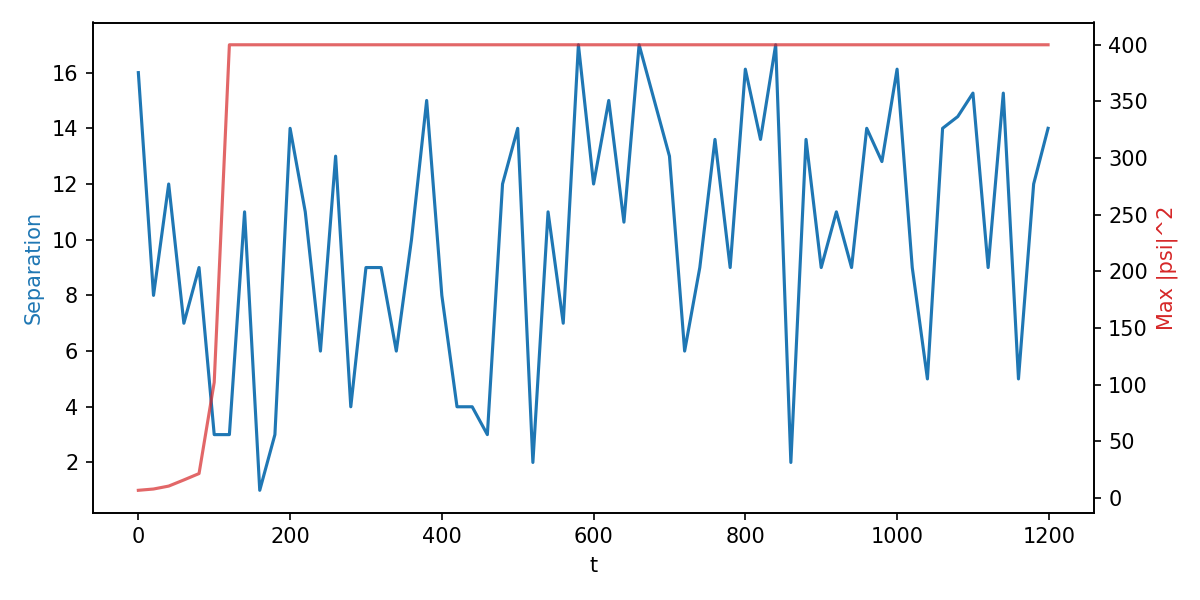
\includegraphics[width=0.95\textwidth]{figures/session26_unified_timeseries.png}
  \caption{Unified time-series from PR-0 Session 26, showing field evolution, separation dynamics, and emergent force parameter discovery under constraint-conditioned D-minimization. The convergence to stable configurations with low dissonance D demonstrates the efficacy of the annealed PT surrogate in discovering coherent, binding dynamics. From Ref.~\cite{SpivackSDS_PR0}, reproduced with permission.}
  \label{fig:pr0-unified-timeseries}
\end{figure}

For detailed parameter traces, correlation scatter plots (D-$\Phi$ with r=-0.91), energy balance diagnostics, and complete field evolution animations, see the companion PR-0 validation paper~\cite{SpivackSDS_PR0}.

% End of Appendix I

